\documentclass[12pt]{article}
        

\usepackage{amsmath}  				
\usepackage{caption} 
\usepackage{color} 
\usepackage{comment}
\usepackage{fancyhdr}
\usepackage{float}
\usepackage{graphicx} 
\graphicspath{ {Figures/} } 
\usepackage{hyperref}
\usepackage{indentfirst} 
\usepackage{listings}
\usepackage{listings}
\usepackage{longtable}
\usepackage{setspace}     
\usepackage{subcaption}
\usepackage[superscript]{cite}    
\usepackage{cite}
\usepackage{titlesec}
\usepackage[normalem]{ulem}  
\usepackage{url}
\usepackage[table]{xcolor}
\usepackage{makecell}
\usepackage{graphicx}
\graphicspath{ {./images/} }

\textwidth=6.5in                    
\oddsidemargin=0.0in    
\pagestyle{fancy}
\fancyhf{}
\lhead{Family Organization }
\rhead{Page \thepage}

  

\hypersetup{
    colorlinks=true,
    citecolor=black,
    linktoc=all, 
    linkcolor=black,
}
\titlespacing*{\subsection}
{0pt}{1pt}{1pt}

\begin{document}

\begin{titlepage}

\newcommand{\HRule}{\rule{\linewidth}{0.5mm}} 

\center 

\textsc{\LARGE Missouri State University\\~\\Department computer Science}\\[1.0cm] 

\HRule \\[0.4cm]
{ \huge \bfseries Family Organization}\\[0.4cm] 
\HRule \\[1.5cm]



\begin{minipage}{0.4\textwidth}
\begin{flushleft} \large
Adam Barnes \\ Dala Biart \\ Kyle Chrzanowski \\ Matt Lippelman \\ 
\end{flushleft}
\end{minipage}
~
\begin{minipage}{0.4\textwidth}
\begin{flushright} \large
Mohammed Belkhouche \\ 
YassineBelkhouche@MissouriState.edu
\end{flushright}
\end{minipage}\\[2cm]

{\large \today}\\[2cm] 

\end{titlepage}

\newpage
%-----------------------------------------------------------------------
\tableofcontents

\newpage
%----------------------------------------------------------------------

%-----------------------------------------------------------------------------
\section {Family Organization}
\subsection{Software Description}
Our project is a family organization and interaction application. It is a web application meant to keep track of different 
kinds of applications a family would need to stay organized, whether that be meal planning, creating a shopping list, or just keeping track of 
family events. Each functionality is meant to be customized to fit the users' needs. The app will have to add "authorization" to offer security to the users, ensuring that important knowledge and data stays within the family. The application will be able to be scaled through additional modules with different functionalities, as we don't yet know how big the project will become. Modules are listed and explained below, with modules we believe we can feasibly implement
in the allotted time under section 2 and any additional proposed modules listed under section 3.

\section{Functions}
\subsection{Basic Functionality}
\begin{itemize}
    \item Basic authentication with email and password
    \item User will be able to create a family entity
    \item User will be able to add other users to their family
    \item User will be able to assign family roles to members of their family
    \item Users will only be able to access data for their own family
\end{itemize}
\subsection{Proposed Modules}
\begin{itemize}
    \item To-Do List: A To-Do list for each person in the family, to-dos will be colored to represent
            the different family members. Ability to create, read, update, and delete tasks will be included.
            Proposed module would have filters for viewing specific tasks or viewing other family member's tasks.
    \item Calendar: A calendar of all family events and individual events. We picture this module being particularly
            helpful in keeping track of the extra curricular activities that children have as well as planning
            family meetings, etc. Like the to-do list, the calendar events should be color coded per family member
            for a better user experience when viewing the calendar and filters should be included. The Calendar should have 
            the ability to create, read, update, and delete calendar events.
    \item Polling App: Members of a family can create polls for other family members to participate in. We see this being
            used for things like planning family events, picking a movie for a family night, picking out meals to eat for
            the week from a list of possibilities, etc. 
    \item Shopping List: A simple list of items to get while at the store. Members of the family should be able to add
            to the list, remove items from the list, and update items. This should be a list of items with the corresponding
            quantities.
\end{itemize}

\begingroup
\section{Extra Functions (if we have extra time)}
\subsection{Proposed Modules}
\begin{itemize}
    \item Meal Planner: For the Meal Planner module, the user would be presented with a 7 day calendar view where they can
            plan meals for the week. This could work with the shopping list with the ability to export the ingredients needed
            for each meal to the shopping list with appropriate quantities. We see users having the ability to add their own recipes
            as well as publish them to be used by other families.
    \item Family Chat: The Family Chat module would be a simple group chat feature, where families can have a conversation that 
            doesn't clog up their SMS inboxes as well as be available to family members without phone access.
    \item Shared File Uploads: With this module, family members would have the ability to upload files that others in the family
            would be able to access. It could be anything from a shared photo album to a vacation itinerary.
\end{itemize}
\section{Functional Requirements}
    \addcontentsline{toc}{subsection}{FR.1}
    \subsection*{FR.1}
    \begin{center}
        \begin{tabular}{| p{10em} p{26em} |}
        \hline
         Function &  The system must provide user registration\\
         Description & User should be able to sign up with a username, password and app pertinent data. \\
         Inputs & Username, password, email, name\\
         Source & Form fields populated by user\\
         Outputs & None\\
         Action & User is presented with a form to register with the application. Data is submitted to the server to create a user record in the database.\\
         Error Handling & If a record exists with the username or email, an exception will be thrown. The error should be displayed to the user asking for a different value.\\
         Precondition & User does not exist with identifying information\\
         Postcondition & User is created with information provided\\
         Side Effects & None \\
         Related Requirements & FR.2, FR.3\\
         \hline
        \end{tabular}
    \end{center}
    \addcontentsline{toc}{subsection}{FR.2}
    \subsection*{FR.2}
    \begin{center}
        \begin{tabular}{| p{10em} p{26em} |}
        \hline
         Function & The system must provide user authentication\\
         Description & User should be able to sign in with username and password.\\
         Inputs & Username, password\\
         Source & Form fields populated by user\\
         Outputs & A session with a session ID granting access to authenticated users.\\
         Action & User is presented with a form to sign in. Data is submitted to the server to login the user. Upon successful authentication, a session is created and stored in the database. \\
         Error Handling & If the user provided credentials are incorrect a 401 http code will be returned. User should be notified credentials were incorrect.\\
         Precondition & Unauthenticated user. Access to application prevented\\
         Postcondition & User authenticated, session created, and access allowed\\
         Side Effects & None \\
         Related Requirements & FR.1, FR.3\\
         \hline
        \end{tabular}
    \end{center}
    \addcontentsline{toc}{subsection}{FR.3}
    \subsection*{FR.3}
    \begin{center}
        \begin{tabular}{| p{10em} p{26em} |}
        \hline
         Function & The system must allow a user to delete their data.\\
         Description & Users should be able to delete their account and any related data. This action should be authenticated to ensure only the user requesting can delete their user.\\
         Inputs & username, password\\
         Source & Form fields populated by user\\
         Outputs & None\\
         Action & User is prompted to re-authenticate. Request is sent to server with credentials to delete the user. Upon successful authentication, the user is deleted from the database and is removed from any families.\\
         Error Handling & If authentication fails, server will return a 401 http status, and an appropriate message should be presented to the user.\\
         Precondition & User exists in the database and has access to resources\\
         Postcondition & User and all related data no longer exists and access is removed\\
         Side Effects & Families the user is owner of will be deleted. (To prevent, ownership should be transferred before account deletion)\\
         Related Requirements & FR.2, FR.1\\
         \hline
        \end{tabular}
    \end{center}
    \addcontentsline{toc}{subsection}{FR.4}
    \subsection*{FR.4}
    \begin{center}
        \begin{tabular}{| p{10em} p{26em} |}
        \hline
         Function & The system must allow creation of a family\\
         Description & Users should be able to create a family entity \\
         Inputs & Family name, timezone, all member event color\\
         Source & Form fields populated by user\\
         Outputs & A family entity with appropriate modules created\\
         Action & User is presented with a form to choose a name, timezone, and color picker. Data is submitted to the server to create a family.\\
         Error Handling & If there is an error creating the family record in the database a 500 error will be thrown from the server. UI should present an appropriate message and ask user to resubmit.\\
         Precondition & Family entity does not exist\\
         Postcondition & Family entity has been created\\
         Side Effects & None\\
         Related Requirements & FR.5\\
         \hline
        \end{tabular}
    \end{center}
    \addcontentsline{toc}{subsection}{FR.5}
    \subsection*{FR.5}
    \begin{center}
        \begin{tabular}{| p{10em} p{26em} |}
        \hline
         Function & The system must allow addition of family members\\
         Description & Users should be able to invite other users to become part of their family\\
         Inputs & Username/email of user to invite, and family id to add user to\\
         Source & Username/email supplied through form by user, family id provided from vue store\\
         Outputs & Email to user invited if they exist, nothing if user does not exist\\
         Action & User asked to supply email or username for user to invite. Email sent with active family id to server. If username is provided, a lookup to get email will be done. Email will be sent to user with invite code. No indication of user existing will be returned to requesting user. Alternative to email invite is through unique family invite code that user can share. Invited user inputs invite code into form and is added to family with invite code.\\
         Error Handling & Errors will not be presented to requesting user. If invited user uses an invalid invite code, a 400 http code will be returned from the server, and an appropriate message should be presented to user\\
         Precondition & User is not part of the family\\
         Postcondition & User is invited to family. If join is requested, user is added to family.\\
         Side Effects & \\
         Related Requirements & FR.4, FR.6\\
         \hline
        \end{tabular}
    \end{center}
    \addcontentsline{toc}{subsection}{FR.6}
    \subsection*{FR.6}
    \begin{center}
        \begin{tabular}{| p{10em} p{26em} |}
        \hline
         Function & The system must be able to send invites via email\\
         Description & Upon receipt of an invite request from a user, the system should send an email inviting another user to join a family with a unique invite code. If the user is not already a member, the user will be asked to create an account before joining the family.\\
         Inputs & Email address of user, invite code\\
         Source & Email address will provided by inviting user or will be retrieved from database based on username provided by requesting user. Invite code will be generated on the server side.\\
         Outputs & Email to invited user.\\
         Action & Invite request is received. Invite code is generated. Email is sent to invited user with invite code.\\
         Error Handling & If an invalid email is sent, the server will respond with 400 http status.\\
         Precondition & The invite code does not exist\\
         Postcondition & An invite code is generated and sent to the user.\\
         Side Effects & None\\
         Related Requirements & FR.5, FR.7\\
         \hline
        \end{tabular}
    \end{center}
    \addcontentsline{toc}{subsection}{FR.7}
    \subsection*{FR.7}
    \begin{center}
        \begin{tabular}{| p{10em} p{26em} |}
        \hline
         Function & The system must accept an invite code to join a family\\
         Description & A user should be able to enter an invite code received either via email or from the owner of a family and join a family.\\
         Inputs & Username, invite code, and event color\\
         Source & Username will come from the vue store after the user has logged in, the invite code and user event color will be submitted through a form field\\
         Outputs & None\\
         Action & User is presented with a form to enter the invite code and a color picker to pick an event color for their events in the family. Data is submitted to the server and an entry is created linking the user to the family.\\
         Error Handling & If an invite code that is not valid is received by the server, the server should return a 400 http response. An appropriate error message should be displayed to the user.\\
         Precondition & The invited user is not linked to the family\\
         Postcondition & The invited user has been linked to the family\\
         Side Effects & None\\
         Related Requirements & FR.6, FR.5, FR.4\\
         \hline
        \end{tabular}
    \end{center}
    \addcontentsline{toc}{subsection}{FR.8}
    \subsection*{FR.8}
    \begin{center}
        \begin{tabular}{| p{10em} p{26em} |}
        \hline
         Function & The system must allow family role assignment\\
         Description & A family admin should be able to assign roles to members after they have joined the family. Family roles should be one of: FAMILY\_ADMIN, ADULT, CHILD. FAMILY\_ADMIN should have the highest authority and should be authorized to perform all tasks excluding family setting management. ADULT role should be authorized to edit all events created in the family, including removing them. CHILD role should be able to edit only events they create and items added to lists should require approval by a user with ADULT or higher privileges.\\
         Inputs & Username, role\\
         Source & Form field values from user requesting change\\
         Outputs & None\\
         Action & User will be presented with a list of users and their current roles in the family. User edits role and saves changes. Changes are received on the server and roles updated in the database.\\
         Error Handling & If there is an error processing the request a 500 http respsonse will be sent from the server. An appropriate message should display to the user.\\
         Precondition & User with prechange role\\
         Postcondition & User with edited role is saved to database\\
         Side Effects & Privileges will either be added or removed depending on edited role\\
         Related Requirements & FR.4, FR.5\\
         \hline
        \end{tabular}
    \end{center}
    \addcontentsline{toc}{subsection}{FR.9}
    \subsection*{FR.9}
    \begin{center}
        \begin{tabular}{| p{10em} p{26em} |}
        \hline
         Function & The system must allow ownership transfer of family\\
         Description & User should be able to transfer ownership to another user in the family. This request should be authenticated to ensure only the current family owner can perform this task.\\
         Inputs & Authenticated user, family id, username to transfer to\\
         Source & Form fields populated by user\\
         Outputs & None\\
         Action & User selects user to transfer to, family id is added to request from vue store, and user authenticates via username and password. Data is submitted to the server where the transfer of ownership occurs.\\
         Error Handling & If there is an error authenticating, a 401 response is returned. If there is an error processing the request, a 500 response is returned. An appropriate message should be displayed to the user.\\
         Precondition & Ownership of family belongs to current owner.\\
         Postcondition & Ownership of family is transferred to requested user.\\
         Side Effects & Original owner of family will change to FAMILY\_ADMIN role without ownership privileges.\\
         Related Requirements & FR.3, FR.5, FR.8\\
         \hline
        \end{tabular}
    \end{center}
    \addcontentsline{toc}{subsection}{FR.10}
    \subsection*{FR.10}
    \begin{center}
        \begin{tabular}{| p{10em} p{26em} |}
        \hline
         Function & The system should allow users to belong to multiple families\\
         Description & Users should be able to create and join as many families as they would like.\\
        \makecell{Inputs \\ Source \\ Outputs \\ Action \\ Error Handling \\ Precondition \\ Postcondition \\ Side Effects}
         & If creating, same as FR.4. If joining, same as FR.7\\
         Related Requirements & FR.4, FR.7\\
         \hline
        \end{tabular}
    \end{center}
    \addcontentsline{toc}{subsection}{FR.11}
    \subsection*{FR.11}
    \begin{center}
        \begin{tabular}{| p{10em} p{26em} |}
        \hline
         Function & The system should allow "CRUD" features of to-do items\\
         Description & Users should be able to create, read, update, and delete to-dos. The to-do should be added to the family to-do list in the case of creation and removed in the case of deletion.\\
         Inputs & Data to create/update a new to-do. Id of to-do if request is to delete.\\
         Source & Form fields populated by user.\\
         Outputs & Updated list of to-dos.\\
         Action & User is presented with a form to create or update a to-do. User fills out fields and data is submitted to the server. Server creates or updates the to-do, and an updated list of to-dos is returned. If delete request is sent, to-do is deleted and update list returned.\\
         Error Handling & If an error occurs while processing a to-do operation request, a 500 response is returned. If the user is not authorized to update/delete the to-do, a 401 status will be returned. An appropriate message should be displayed to the user.\\
         Side Effects & Any user with a list of data from before changes will have stale data.\\
         Related Requirements & None.\\
         \hline
        \end{tabular}
    \end{center}
     \addcontentsline{toc}{subsection}{FR.12}
    \subsection*{FR.12}
    \begin{center}
        \begin{tabular}{| p{10em} p{26em} |}
        \hline
         Function & The system should allow CRUD features of calendar events\\
         Description & Users should be able to create, read, update, and delete a calendar event. The event should be added to the family calendar in the case of creation and removed in the case of deletion.\\
         Inputs & Data to create/update a new calendar event. Id of calendar event if request is to delete.\\
         Source & Form fields populated by user.\\
         Outputs & Updated list of calendar events.\\
         Action & User is presented with a form to create or update a calendar event. User fills out fields and data is submitted to the server. Server creates or updates the calendar event, and an updated list of events is returned. If delete request is sent, event is deleted and update list returned.\\
         Error Handling & If an error occurs while processing a calendar event operation request, a 500 response is returned. If the user is not authorized to update/delete the event, a 401 status will be returned. An appropriate message should be displayed to the user.\\
         Side Effects & Any user with a list of data from before changes will have stale data.\\
         Related Requirements & None.\\
         \hline
        \end{tabular}
    \end{center}
    \addcontentsline{toc}{subsection}{FR.13}
    \subsection*{FR.13}
    \begin{center}
        \begin{tabular}{| p{10em} p{26em} |}
        \hline
         Function & The system should allow assignment of to-dos and calendar events to multiple users.\\
         Description & Users should be able to assign multiple users to a calendar event and to-do list items. If multiple users are assigned, the visual color indicator should reflect multiple assignees. If the entire family is assigned, family color should be used.\\
         Inputs & Id of event/to-do, usernames to assign\\
         Source & Form field data supplied by user.\\
         Outputs & Updated list of calendar events/to-dos.\\
         Action & User edits a calendar event/to-do and adds/removes one or more users as assignees. User saves changes and data is submitted to server. Server updates database to reflect changes and returns updated list.\\
         Error Handling & If an error occurs while processing a calendar event/to-do operation request, a 500 response is returned. If the user is not authorized to update/delete the event, a 401 status will be returned. An appropriate message should be displayed to the user.\\
         Precondition & Zero or more assigned people exist on the calendar event/to-do\\
         Postcondition & A different list of assigned people exist on the calendar event/to-do\\
         Side Effects & Any user with a list of data from before changes will have stale data.\\
         Related Requirements & FR.11, FR.12\\
         \hline
        \end{tabular}
    \end{center}
    \addcontentsline{toc}{subsection}{FR.14}
    \subsection*{FR.14}
    \begin{center}
        \begin{tabular}{| p{10em} p{26em} |}
        \hline
         Function & The system should allow filter of calendar events/to-dos.\\
         Description & User should have the ability to filter calendar events/to-dos by user\\
         Inputs & Usernames to include, family id\\
         Source & Usernames received from dropdown selections, family id sent with request from vue store.\\
         Outputs & A list of filtered calendar events/to-dos.\\
         Action & User selects one or more users to filter. Upon focus lost from dropdown, request sent to server. Server processes request and returns list of calendar events/to-dos.\\
         Error Handling & If an error is encountered when processing request, a 500 error response will be returned. An appropriate message should be displayed to the user and current displayed events should remain.\\
         Precondition & Unfiltered events are shown.\\
         Postcondition & Filtered events are shown.\\
         Side Effects & None.\\
         Related Requirements & FR.11, FR.12, FR.13\\
         \hline
        \end{tabular}
    \end{center}
    \addcontentsline{toc}{subsection}{FR.15}
    \subsection*{FR.15}
    \begin{center}
        \begin{tabular}{| p{10em} p{26em} |}
        \hline
         Function & The system should provide CRUD operations for polls.\\
         Description & Users should be able to create a family poll with up to four options. The poll should be sent to all users in the family to vote. Only one vote should be recorded for every user. Poll should not allow updates after any votes are received.\\
         Inputs & Data to create/update a poll. Id of poll if request is to delete.\\
         Source & Form data submitted by user.\\
         Outputs & Updated list of open polls.\\
         Action & User is presented with a form to create or update a poll. User fills out fields and data is submitted to the server. Server creates or updates the poll, and an updated list of poll is returned. If delete request is sent, poll is deleted and update list returned. \\
         Error Handling & If an error occurs while processing a poll operation request, a 500 response is returned. If the user is not authorized to update/delete the poll, a 401 status will be returned. An appropriate message should be displayed to the user.\\
         Side Effects & Any user with a list of data from before changes will have stale data.\\
         Related Requirements & None.\\
         \hline
        \end{tabular}
    \end{center}
    \addcontentsline{toc}{subsection}{FR.16}
    \subsection*{FR.16}
    \begin{center}
        \begin{tabular}{| p{10em} p{26em} |}
        \hline
         Function & The system should allow users of a family to vote in a poll\\
         Description & Users should be able to vote in family polls. Users should be able to update their choice until the poll closes. The user should only record one choice per poll.\\
         Inputs & Poll id, username of voting user, id of choice.\\
         Source & Form fields submitted by the user.\\
         Outputs & Updated poll list.\\
         Action & User opens a poll, chooses an option and submits their choice. Data is submitted to the server and the user's response is recorded. An updated list of polls still open is returned to the user.\\
         Error Handling & If an error occurs while processing a poll operation request, a 500 response is returned. An appropriate message should be displayed to the user.\\
         Side Effects & None.\\
         Related Requirements & FR.15\\
         \hline
        \end{tabular}
    \end{center}
    \addcontentsline{toc}{subsection}{FR.17}
    \subsection*{FR.17}
    \begin{center}
        \begin{tabular}{| p{10em} p{26em} |}
        \hline
         Function & The system should allow users to filter polls.\\
         Description & Users should be able to filter polls by their vote status and poll status. In this instance vote status is defined as whether or not the user has voted on the poll yet. Poll status will either be open or closed. Default view should be polls that are still open with polls not voted on at the top.\\
         Inputs & Poll status, vote status, username, family id.\\
         Source & Poll status and vote status provided through drop down selection. Username and family id provided from vue store.\\
         Outputs & Filtered list of polls.\\
         Action & User selects one or more statuses to filter. Upon focus lost from dropdown, request sent to server. Server processes request and returns list of polls.\\
         Error Handling & If an error occurs while processing a poll filter operation request, a 500 response is returned. An appropriate message should be displayed to the user.\\
         Precondition & Unfiltered polls are shown.\\
         Postcondition & Filtered polls are shown.\\
         Side Effects & None.\\
         Related Requirements & FR.15, FR.16\\
         \hline
        \end{tabular}
    \end{center}
    \addcontentsline{toc}{subsection}{FR.18}
    \subsection*{FR.18}
    \begin{center}
        \begin{tabular}{| p{10em} p{26em} |}
        \hline
         Function & The system should provide CRUD operations for shopping lists\\
         Description & Users should be able to create a shopping list and add/remove items. 
         Items should contain both a description and a quantity needed.\\
         Inputs & Data to create a shopping list item. Id of item and id of list if request is to delete.\\
         Source & Form fields populated by user\\
         Outputs & Updated list of items.\\
         Action & User is presented with a form to add a shopping list item. User fills out fields and data
         is submitted to the server. Server creates an item and sends back an updated list. If update, user
         edits the data or increments/decrements the quantity needed and a request is sent to the server. Server updates the items data and sends back an updated list. If delete, user clicks the delete option of the item. A request is sent to the server, the item is removed from the database, and an updated list is returned.\\
         Error Handling & If an error occurs while processing, a 500 response is returned. If the user is not authorized to add/remove an item, a 401 status will be returned. If the family is not found a 404 response will be returned. An appropriate message should be displayed to the user.\\
         Side Effects & Any user with a list of data from before changes will have stale data.\\
         Related Requirements & None.\\
         \hline
        \end{tabular}
    \end{center}
    \addcontentsline{toc}{subsection}{FR.19}
    \subsection*{FR.19}
    \begin{center}
        \begin{tabular}{| p{10em} p{26em} |}
        \hline
         Function & The system should allow multiple lists per family.\\
         Description & Users should be able to create multiple shopping lists and label them. A default shopping list should be created with the label "Family Shopping List." This list should not be delete-able.\\
         Inputs & A label for the shopping list, and a minimum security level to add/remove/view items from the list.\\
         Source & Form field data supplied by a user.\\
         Outputs & A list of shopping lists.\\
         Action & User fills out a form with the necessary data to create a new shopping list and a request is sent to the server. The server processes the request and sends back the new list of shopping lists.\\
         Error Handling & If an error occurs while processing, a 500 response is returned. If the user is not authorized to add/remove a list, a 401 status will be returned. If the family is not found a 404 response will be returned. An appropriate message should be displayed to the user.\\
         Side Effects & Any user with a list of data from before changes will have stale data.\\
         Related Requirements & FR.18\\
         \hline
        \end{tabular}
    \end{center}
    
\begin{comment}
    \addcontentsline{toc}{subsection}{FR.x}
    \subsection*{FR.x}
    \begin{center}
        \begin{tabular}{| p{10em} p{26em} |}
        \hline
         Function & \\
         Description & \\
         Inputs & \\
         Source & \\
         Outputs & \\
         Action & \\
         Error Handling & \\
         Precondition & \\
         Postcondition & \\
         Side Effects & \\
         Related Requirements & \\
         \hline
        \end{tabular}
    \end{center}
\end{comment}

\section{Non-Functional Requirements}
    \addcontentsline{toc}{subsection}{NFR.1}
    \subsection*{NFR.1}
    \begin{center}
        \begin{tabular}{| p{10em} p{26em} |}
        \hline
         Function & The system should return responses in less than 0.1 seconds\\
         Description & After the user has submitted any request to the server, a response should be returned in less than 0.1 seconds, based on current Web App response time trends.\\
         Inputs & User request data.\\
         Outputs & Response data.\\
         Action & User request is received. Work is completed on the server and a response is returned.\\
         Error Handling & If an error is encountered while processing, an appropriate http error response will be returned from the server. An appropriate error message should be returned.\\
         Related Requirements & FR.1 - FR.17\\
         \hline
        \end{tabular}
    \end{center}
    \addcontentsline{toc}{subsection}{NFR.2}
    \subsection*{NFR.2}
    \begin{center}
        \begin{tabular}{| p{10em} p{26em} |}
        \hline
         Function & The system should have a 0\% failure rate with 500 error code\\
         Description & The server should respond with a 500 error code 0\% of the time. Exceptions should be caught and handled appropriately to prevent 500 error codes. \\
         Inputs & N/A\\
         Outputs & N/A\\
         Action & N/A\\
         Error Handling & Server errors should be caught and dealt with appropriately to prevent server from crashing and returning error code 500.\\
         Related Requirements & FR.1 - FR.17\\
         \hline
        \end{tabular}
    \end{center}
    \addcontentsline{toc}{subsection}{NFR.3}
    \subsection*{NFR.3}
    \begin{center}
        \begin{tabular}{| p{10em} p{26em} |}
        \hline
         Function & The system should have a 0\% data corruption rate upon operation failure.\\
         Description & When an error is encountered while processing a request, necessary steps should be taken to rollback the database commit to prevent data corruption. An appropriate error message should be returned and the user should be asked to resubmit.\\
         Inputs & N/A\\
         Outputs & N/A\\
         Action & N/A\\
         Error Handling & Exception should be caught, commit rolled back, and appropriate message sent to user.\\
         Related Requirements & FR.1 - FR.17, NFR.2\\
         \hline
        \end{tabular}
    \end{center}
    \addcontentsline{toc}{subsection}{NFR.4}
    \subsection*{NFR.4}
    \begin{center}
        \begin{tabular}{| p{10em} p{26em} |}
        \hline
         Function & The system should prevent access to family data to which they are not family members.\\
         Description & Users should only be able to view family data from families they are linked to.\\
         Inputs & User credentials\\
         Outputs & Data requiring authentication\\
         Action & If a user attempts to access data they should not, a 401 http response code should be returned and use should be routed to the previous page they were on or to the login page if not authenticated.\\
         Error Handling & If an authorization issue occurs, a 401 error code should be returned.\\
         Related Requirements & FR.3 - FR.17\\
         \hline
        \end{tabular}
    \end{center}
    \addcontentsline{toc}{subsection}{NFR.5}
    \subsection*{NFR.5}
    \begin{center}
        \begin{tabular}{| p{10em} p{26em} |}
        \hline
         Function & The system should prevent users from accessing data and features their roles do not allow\\
         Description & Users with CHILD access should only be able to create new events/to-dos/polls and edit/delete events/to-dos/polls they created. ADULT role users should be authorized to perform all tasks allowed by a CHILD in addition to editing/deleting events/to-dos/polls of other users in the family. Users with FAMILY\_ADMIN should be authorized to perform all tasks afforded to ADULT role users, and should have the authority to assign roles to other users in the family. Family settings and deletion/transferal of a family should only be accessible by the family owner. Family owners should also have all privileges available to the FAMILY\_ADMIN role.\\
         Inputs & N/A\\
         Outputs & N/A\\
         Action & Appropriate data and features should be hidden from users without access.\\
         Error Handling & If a user attempts to circumvent authorization blocks, a 401 response code should be returned and the request ignored.\\
         Related Requirements & FR.8\\
         \hline
        \end{tabular}
    \end{center}
    
\begin{comment}
    \addcontentsline{toc}{subsection}{NFR.x}
    \subsection*{NFR.x}
    \begin{center}
        \begin{tabular}{| p{10em} p{26em} |}
        \hline
         Function & \\
         Description & \\
         Inputs & \\
         Outputs & \\
         Action & \\
         Error Handling & \\
         Related Requirements & \\
         \hline
        \end{tabular}
    \end{center}
\end{comment}
\section{Architectural Design}
\subsection{Server Architecture}
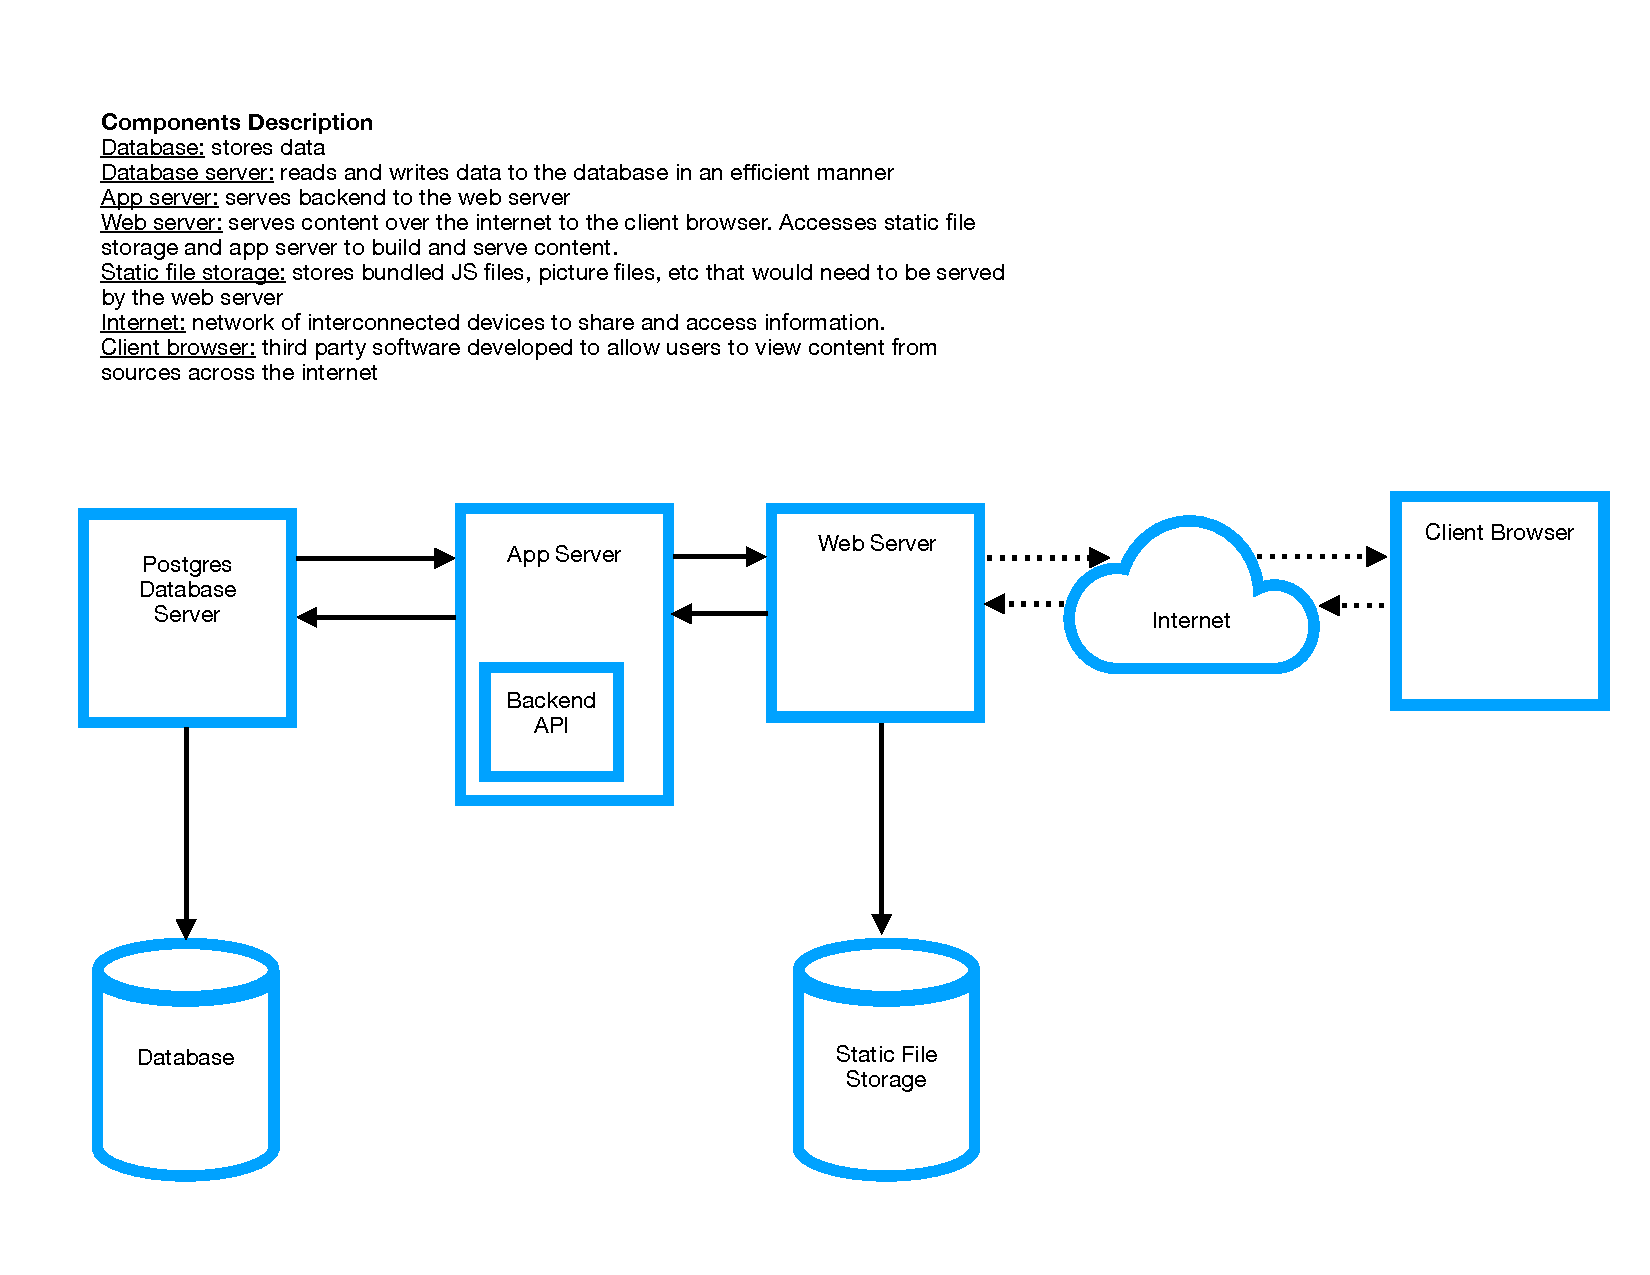
\includegraphics[scale=0.75, angle=90]{Architectural_design}
\subsection{Core}
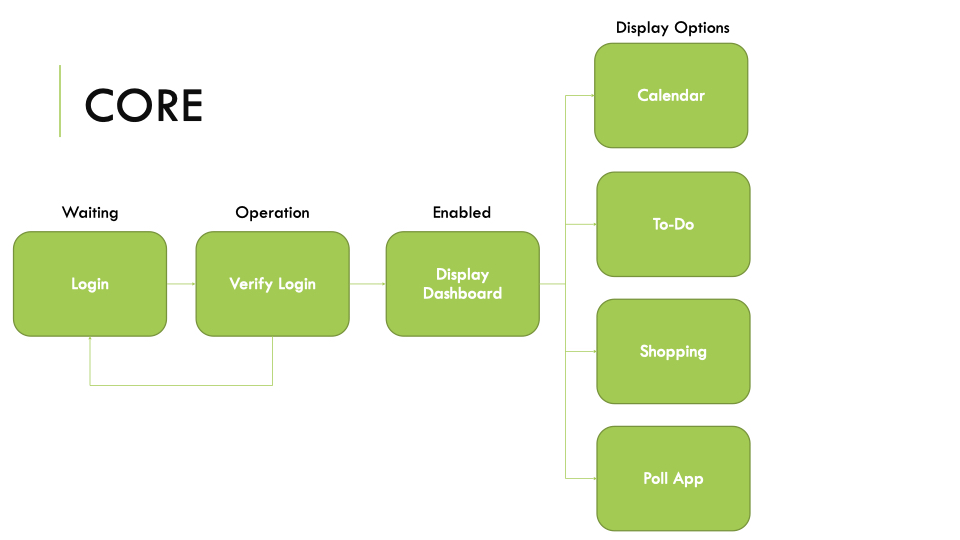
\includegraphics[scale=0.45]{CSC450_Design.001.jpeg}
\subsection{Calendar Module}
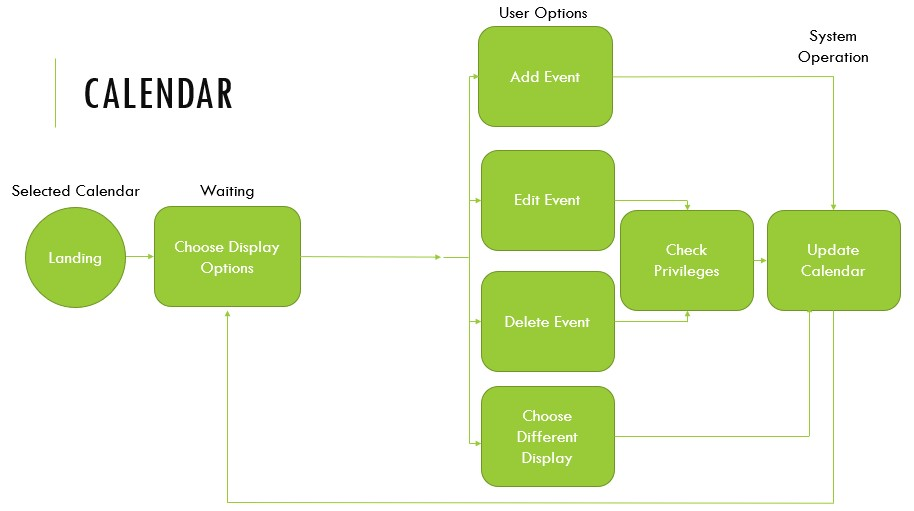
\includegraphics[scale= 0.65]{CSC450_Design.002.jpeg}
\subsection{To-Do List Module}
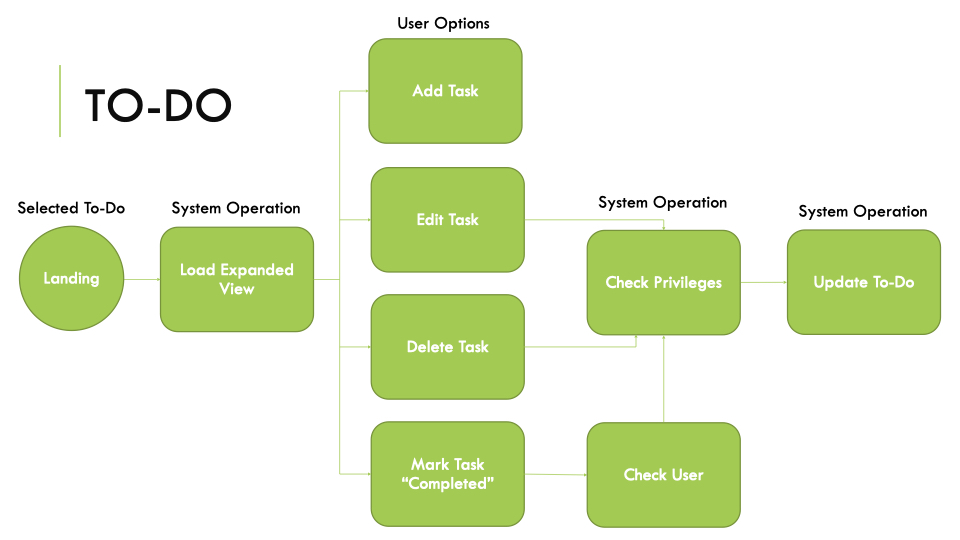
\includegraphics[scale=0.45]{CSC450_Design.003.jpeg}
\subsection{Shopping List Module}
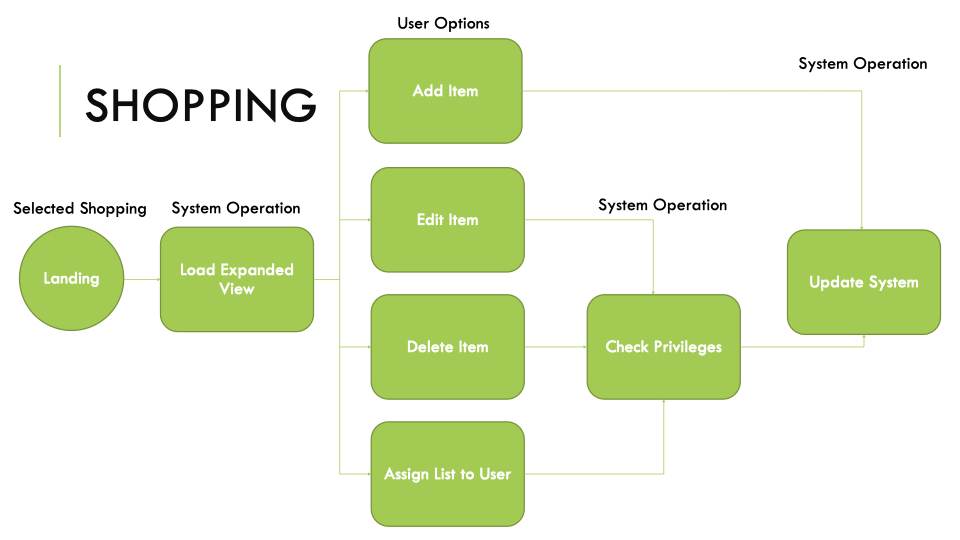
\includegraphics[scale=0.45]{CSC450_Design.004.jpeg}
\subsection{Polling Module}
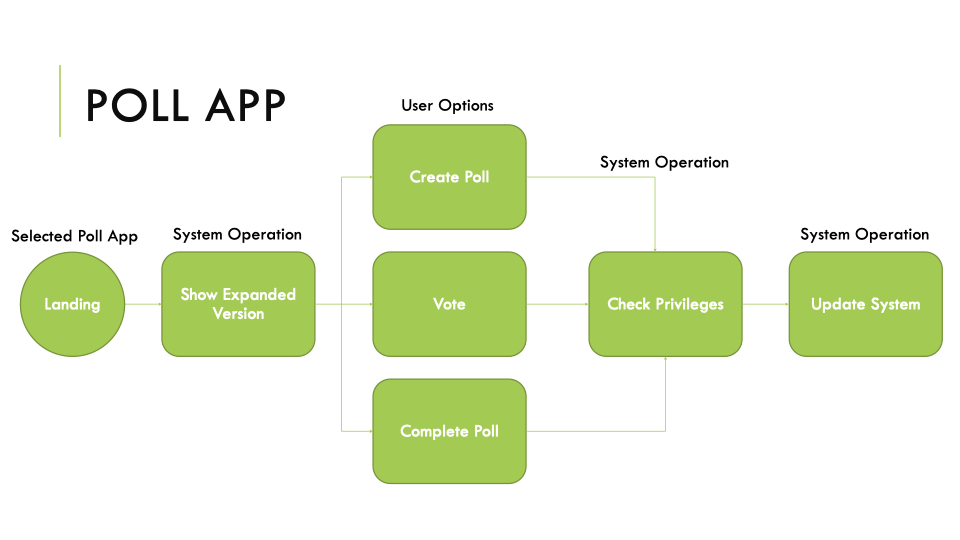
\includegraphics[scale=0.45]{CSC450_Design.005.jpeg}
\section {Implementation and testing}

\subsection{Development environment and tools}
\begin{itemize}
    \item Spring MVC(with Spring Boot): Assists interactions between Model, View, and Controller and their ability to mesh with Spring Boot. 
    \item VueJS: Used to help the Javascript files integrate well with the user components written on the front-end. 
    \item Vuetify: A library of User Interface components to create web applications more easily. 
    \item Vuex: Works as a software library to be used by VueJS and aids in state management. 
    \item Yarn: Package manager for version control between programmers.
    \item Maven: Build manager to simplify building and version control. 
    \item Postgres: The database used to hold Family objects, user information, and data from all of the modules. 
    \item Hibernate:  Object–relational mapping tool used for the Java files to aid in object-oriented programming. 
    \item Mockito: Used for mocking and testing purposes. Creates mock objects to test the Java files used by the back-end.
    \item Jest: Unit testing for use on Javascript programs, ensuring that they integrate with Vue and its related modules. Tests code as it is being written to ensure front-end programs run as intended. 
    \item JUnit: Unit testing to test the functionality of the Java programs in our project as they are being written. Used in regards to programs written on the back-end. 
    \item Cypress testing: Used for end-to-end testing to ensure front-end and back-end can interact as intended. 
\end{itemize}

\subsection{Algorithms used and their description}
\begin{itemize}
    \item BCryptPasswordEncoder: Adaptive hashing algorithm used to encode the password
    \item Built in collection algorithms: Used for sorting, filtering, mapping, etc.
\end{itemize}

\subsection{Reused components}

\begin{itemize}
\subsection{Methods being reused}
    \item CheckPrivileges(): Check role of the user to determine if they have the access to perform a task.
    \item search(): Some modules that can end up being long and difficult to navigate (such as calendar) have a search() function to look for a specific object within the module. 
    
\begin{flushleft} \large
Open source code being reused
\end{flushleft}
    \item SpringMVC: Used to manage Model, View, Controller interactions to ensure it runs with SpringBoot. 
    \item ChartJS: ChartJS is seen in places such as the polling app to visualize data being collected for the family object. 
    \item Vuetify components: Vuetify is used for simple UI functions that we build off of. 
    \item Axios: Used as an http client to interact with the web. 
    \item Vuex Store: Used to manage application state to ensure it runs with the Vue framework. 
\end{itemize}

\section{Testing scenarios and results}
\subsection{Unit Testing}
    We have hundreds of test cases and tests, but have only included a few of the key tests and related test cases to give a basic idea. There are currently plans to make more tests as each module such as shopping list, calendar, and polling.
\begin{itemize}
    \item Sign up: Tested ability to create a new account via the registration page. Sign up works for any user, regardless of whether or not they have a family invite code. 
    \item Password validation: Checking the standards for the passwords of new users. Inserted several different inputs in the password field on the user registration page. Criterion we settled on for passwords is as follows: \\
    -Only accept the input if it had between 12-32 characters \\
    -At least one lowercase and uppercase letter \\
    -At least one number \\
    -At least one special character 
    \item Password confirmation: Checking the ability to log in for an existing user. Attempted submitting the registration form with passwords that did not match. It did not allow submission and displayed an error
    \item Creation of a family object: Creating a family object makes you the admin of said family. It also allows you to generate an invite code which can be sent to new or existing users. 
    \item Deleting an item from the shopping list: Removed an object from a shopping list by selecting the delete icon. The item the disappeared from the list.
    \item Account deletion: Wanted to check if the data for the account was properly deleted when done so in the user settings. We created and then deleted a user account. Accessed the database to confirm the account and the data associated with it was gone
    \item Child role privileges: Tests using a child account to ensure children do not have abilities to delete items such as tasks, events, or family objects. Checked to make sure the child role’s restrictions worked as intended. Attempted several deletion events with an account that has a Child role in a family. Ability to delete a family, list, or event is not available for the child role.
    \item Adult role privileges: Adult role has more privileges than the Child role but does not have admin access to the family account. Tested with a mock adult account to ensure that users with the Adult role could interact with the modules and had the ability to create, edit and delete. Adults do not have the option to generate a registration code for the family object, nor do they have the ability to create polls.  
    \item Admin role privileges: Admin role has the most privileges and is most likely the user who created the family object. Tested to ensure they have the ability to edit family objects. Also tested generation of registration codes by sending an invite to a different account, which allows the addition of a new user to the family object. 
    \item Admin role privileges: Admin role has the most privileges and is most likely the user who created the family object. Tested to ensure they have the ability to create, edit, and delete family objects. Also tested generation of registration codes by sending an invite to a different account, which allows the addition of a new user to the family object.
    \item Creating a poll: Permissions are only granted to the owner of a family account to create a poll. Other users in that family, regardless of role, can interact and vote on that poll before the set end time of voting. 
\end{itemize}


\subsection{Integration Testing}
Integration testing is handled via open source software we use. This ensures that code is always being tested as we are writing it. SpringMVC ensures that interactions run smoothly between the Model, View, and Controller. Jest and JUnit respectively are used to ensure Javascript and Java files can be tested before running them. Any of the software we use will throw errors if they did not integrate well with our current program. 

\subsection{Test Cases}
\begin{itemize}
    \item Email: dbiart.47@gmail.com \\ Name: Jim ChildRole \\ Role: Child \\ Family: ChildRole Family \\ The goal is of this role is to ensure that child role functions as intended. 
    \item Email: beesdoingart01@gmail.com \\ Name: Tim AdultRole \\ Role: Adult \\ Family: AdultRole Family \\ The goal is of this role is to ensure that adult role functions as intended. 
    \item Email: Biart23@live.MissouriState.edu \\ Name: GimGam AdminRole \\ Role: Admin \\Family: AdminRole Family \\ The goal is of this role is to ensure that admin role functions as intended.
    \item Calendar event: Take Jim ChildRole to soccer practice \\ Recurring: Yes \\ Time: 4:30pm \\ Date: Every Tuesday & Thursday \\ To ensure calendar can run recurring events.
    \item To do list: Mow the lawn \\ Appears on the user: Tim AdultRole \\ To test to do list's ability to create, edit and delete tasks. 
    \item Shopping List: Buy milk, eggs, and butter \\ To test shopping list's ability to create, edit, and delete. 
\end{itemize}

\end{document}
